\chapter{Environment and Tooling}

\section{Test Environment Overview}

\noindent
The practical exploitation work requires a \textbf{controlled, reproducible test environment} that supports \textbf{eBPF program loading}, \textbf{XDP attachment}, \textbf{packet generation}, and \textbf{kernel tracing}. Our environment is built on \textbf{Linux LTS 6.8} running inside a \textbf{KVM/QEMU virtual machine} with 2 vCPUs, 4 GB of RAM, and a 20 GB virtual disk. The base image is \textbf{Ubuntu 24.04 (Noble) Cloud Image}, chosen for its balance of stability, standardization, and tooling availability. This configuration ensures that any finding can be \textbf{reproduced on an identically configured system}.

\begin{figure}[h]
\centering
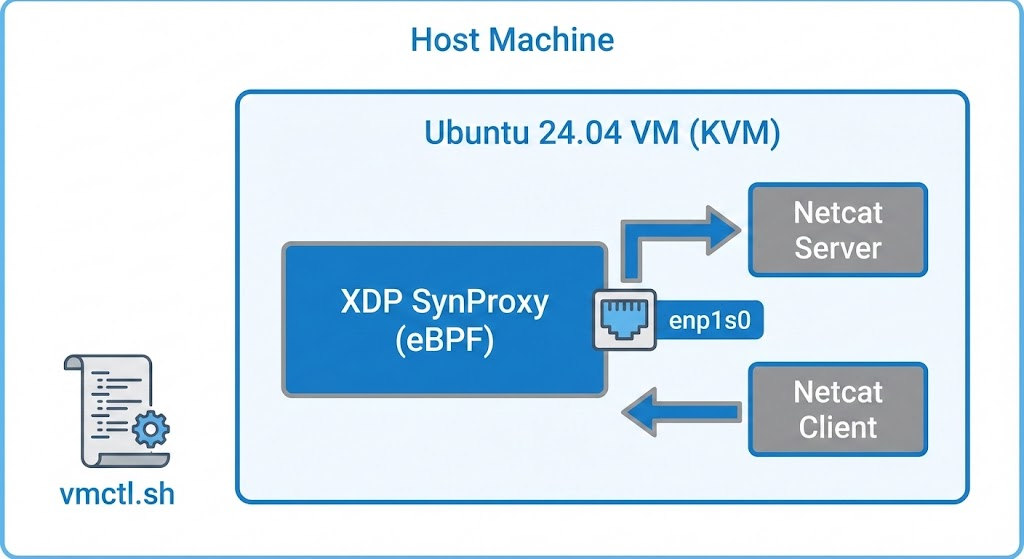
\includegraphics[width=0.7\textwidth]{resources/images/VM_Structure.jpg}
\caption{VM Architecture: Isolated test environment for safe vulnerability exploitation (diagram by author)}
\end{figure}

\subsection{VM Lifecycle Management}

\noindent
The \textbf{virtual machine infrastructure} was created by the \textbf{previous research team} and included a \texttt{virt/vmctl.sh} script that automates \textbf{VM creation}, \textbf{provisioning}, \textbf{connection}, and \textbf{teardown}. For this work, we made \textbf{some modifications and enhancements} to the original setup, as detailed in Section 4 (Infrastructure Modifications to Inherited Codebase).

\noindent
To create and provision a VM, an operator invokes the script with their SSH public key, and \textbf{cloud-init} automatically installs all necessary dependencies with our enhancements. \textbf{SSH access} to the VM is passwordless, facilitating automated testing pipelines. The script also provides a \texttt{connect} subcommand for interactive debugging and a \texttt{destroy} subcommand for cleanup.

\vspace{0.3cm}
\noindent
For convenience, we created a \textbf{Makefile} in the root of the repository that wraps the underlying \texttt{vmctl.sh} script, providing \textbf{three simple commands} for VM management:

\begin{itemize}
  \item \textbf{\texttt{make create}}: Runs the complete VM provisioning workflow, including download of the base image, VM creation, and cloud-init setup. The script executes until it prompts for SSH key credentials. For this test environment, we used basic credentials: username \texttt{ubuntu} and password \texttt{u} for expedited testing.
  \item \textbf{\texttt{make connect}}: Establishes an interactive SSH connection to the running VM for debugging and manual inspection.
  \item \textbf{\texttt{make destroy}}: Powers down and permanently deletes the VM, cleaning up disk space and libvirt configurations.
\end{itemize}

\vspace{0.3cm}
\noindent
This abstraction eliminates the need to remember or manually invoke \texttt{vmctl.sh} paths and parameters, streamlining the VM lifecycle during exploitation testing.

\noindent
VM provisioning via cloud-init installs a \textbf{comprehensive development environment}: the \textbf{clang} and \textbf{llvm} compilers for eBPF bytecode generation, \textbf{bpftool} for kernel interaction, \textbf{linux-headers} matching the kernel version, \textbf{network utilities} (netcat, tcpdump, iproute2), \textbf{build tools} (make, git, gcc), and configures \textbf{SSH key injection} for passwordless access. This ensures the VM is ready for testing immediately after creation.

\vspace{0.3cm}
\noindent
Additionally, we configured a \textbf{shared folder} between the host machine and the guest VM, mounted at \texttt{/mnt/shared} in the VM or at \texttt{/home/ubuntu/shared}. This shared directory allows \textbf{seamless transfer} of exploit payloads, proof-of-concept scripts, and compiled binaries from the host to the VM without requiring manual SCP transfers, streamlining the iterative testing workflow.

\subsection{Network Configuration for XDP and External Exploitation}

\noindent
\textbf{XDP program attachment} requires a \textbf{real Ethernet interface} (not virtual) so that packets are processed at the \textbf{driver level} before entering the kernel's normal networking stack. The test environment configures the VM with \textbf{Layer 2 connectivity} to the host via \textbf{bridge networking}, a standard MTU of 1500 bytes, and \textbf{promiscuous mode} enabled on the XDP-attached interface. This configuration allows the test harness running on the host to send \textbf{arbitrary packets} to the VM's interface and observe the XDP program's processing.

\noindent
The key innovation is the \textbf{external-perspective exploitation}: rather than triggering vulnerabilities from within the VM itself, we deploy exploit code on the host machine that targets the VM's network interface over the network boundary. This setup provides a \textbf{real-world exploitation scenario} where an unprivileged attacker sends crafted TCP packets from an external source (the host) to an eBPF program running on a network-attached server (the VM). This approach better models realistic attack conditions than local-only exploitation, demonstrating that eBPF verifier failures can be exploited from a network-adjacent attacker position.

\section{Compilation Pipeline}

\noindent
The \textbf{eBPF compilation process} follows a \textbf{multi-stage approach} to ensure vulnerabilities survive from source code through to kernel execution.

\subsection{C to eBPF Bytecode}

\noindent
The standard invocation using \textbf{clang} is:

\vspace{0.3cm}
\noindent
\fcolorbox{black!30}{gray!15}{%
  \begin{minipage}[c]{\dimexpr\textwidth-2\fboxsep-2\fboxrule}
    {\small\ttfamily
    clang -O2 -target bpf -c xdp\_synproxy\_kern.c -o xdp\_synproxy\_kern.o
    }
  \end{minipage}%
}
\vspace{0.3cm}

\noindent
The \textbf{-O2} optimization level is critical because \texttt{-O0} may preserve temporary variables and memory operations that the optimizer would normally eliminate. The \textbf{-target bpf} flag directs compilation to the eBPF instruction set rather than the native host architecture (x86-64, ARM, etc.). The \textbf{-c} flag produces an object file without linking, since eBPF programs are self-contained units without external symbol dependencies.

\subsection{Bytecode Inspection with llvm-objdump}

\noindent
After compilation, we \textbf{inspect the bytecode} to confirm the \textbf{vulnerable code path is present} and was not optimized away:

\vspace{0.3cm}
\noindent
\fcolorbox{black!30}{gray!15}{%
  \begin{minipage}[c]{\dimexpr\textwidth-2\fboxsep-2\fboxrule}
    {\small\ttfamily
    llvm-objdump -d xdp\_synproxy\_kern.o > bytecode\_analysis.txt
    }
  \end{minipage}%
}
\vspace{0.3cm}

\noindent
This inspection reveals the \textbf{full instruction sequence} in the vulnerable function, \textbf{register usage patterns}, \textbf{memory access operations} (loads and stores), and \textbf{bounds checks or arithmetic} that might be relevant to the vulnerability. This step is essential to prove that the compiler did not inadvertently eliminate the vulnerability through dead-code elimination or aggressive optimization.

\section{Kernel Tools and eBPF Loading}

The bpftool utility is the primary interface for interacting with loaded eBPF programs. To load a compiled eBPF object file and capture verifier diagnostics, we use:

\vspace{0.3cm}
\noindent
\fcolorbox{black!30}{gray!15}{%
  \begin{minipage}[c]{\dimexpr\textwidth-2\fboxsep-2\fboxrule}
    {\small\ttfamily
    bpftool prog load xdp\_synproxy\_kern.o /sys/fs/bpf/my\_prog \\
    \ \ type xdp verbose 2>\&1 | tee verifier.log
    }
  \end{minipage}%
}
\vspace{0.3cm}

\noindent
The \texttt{verbose} flag is essential; it causes the kernel to output the verifier's complete internal reasoning, including the register types and ranges tracked at each instruction, the constraints on memory offsets, and the specific reasoning for any rejection. These logs are piped to a file for post-analysis and evidence documentation.

After successful loading, attaching the program to a network interface is straightforward:

\vspace{0.3cm}
\noindent
\fcolorbox{black!30}{gray!15}{%
  \begin{minipage}[c]{\dimexpr\textwidth-2\fboxsep-2\fboxrule}
    {\small\ttfamily
    ip link set dev enp2s0 xdp obj xdp\_synproxy\_kern.o sec .text
    }
  \end{minipage}%
}
\vspace{0.3cm}

\noindent
Packets arriving on \texttt{enp2s0} are now processed by the eBPF program at the driver level, before entering the kernel's normal networking stack. This is the execution point where vulnerabilities manifest.

Post-verification, the kernel performs internal bytecode transformations and optimizations. These can be inspected via the \textit{xlated} dump:

\vspace{0.3cm}
\noindent
\fcolorbox{black!30}{gray!15}{%
  \begin{minipage}[c]{\dimexpr\textwidth-2\fboxsep-2\fboxrule}
    {\small\ttfamily
    bpftool prog dump xlated name my\_prog > xlated.dump
    }
  \end{minipage}%
}
\vspace{0.3cm}

\noindent
The xlated dump shows the bytecode as it exists in kernel memory after the verifier has processed it. This proves whether the vulnerability survived verification intact or was transformed/sanitized. Runtime traces and kernel output confirm execution and behavior.

\section{Runtime Observation and Debugging}

\subsection{Kernel Tracing with trace\_pipe}

eBPF debug output uses the \texttt{bpf\_printk} macro, which writes messages to the kernel trace buffer. These can be observed in real-time via:

\vspace{0.3cm}
\noindent
\fcolorbox{black!30}{gray!15}{%
  \begin{minipage}[c]{\dimexpr\textwidth-2\fboxsep-2\fboxrule}
    {\small\ttfamily
    cat /sys/kernel/debug/tracing/trace\_pipe
    }
  \end{minipage}%
}
\vspace{0.3cm}

\noindent
During PoC execution, trace output confirms that specific code paths are executing and vulnerabilities are being triggered. Example output from vulnerability testing:

\vspace{0.3cm}
\noindent
\fcolorbox{black!30}{gray!15}{%
  \begin{minipage}[c]{\dimexpr\textwidth-2\fboxsep-2\fboxrule}
    {\small\ttfamily
    \texttt{[argcomp]: 5.6a - csum}\\
    \texttt{[taintnoproto]: 5.39 - OOB index: 18}\\
    \texttt{[taintsink]: 5.46b - Copy length: 256}
    }
  \end{minipage}%
}
\vspace{0.3cm}

\noindent
Each line corresponds to a vulnerability test; the messages confirm that the vulnerable code executed and reached the instrumentation point. This provides immediate feedback during exploitation attempts.

\section{Proof-of-Concept Development}

\subsection{High-Level Packet Crafting with Scapy}

For the \textbf{simpler ABI violation vulnerabilities} (5.06a, 5.06b, 5.06d), PoCs use \textbf{Python with the Scapy library} for straightforward packet construction and sending. A typical exploit:

\vspace{0.3cm}
\noindent
\fcolorbox{black!30}{gray!15}{%
  \begin{minipage}[c]{\dimexpr\textwidth-2\fboxsep-2\fboxrule}
    {\small\ttfamily
    from scapy.all import IP, TCP, send\\
    target\_ip = detect\_vm\_ip()  \# Auto-detect via virsh\\
    pkt = IP(dst=target\_ip) / TCP(dport=80, flags="S")\\
    send(pkt, count=5, verbose=0)
    }
  \end{minipage}%
}
\vspace{0.3cm}

\noindent
This approach offers \textbf{simplicity and automation}: IP and TCP headers are automatically generated, checksums are computed by Scapy, and the packet is sent at the raw layer. Scapy handles the complexity of socket setup and header formatting. All ABI-mismatch PoCs include \textbf{automatic IP detection} using \texttt{virsh} queries to find the target VM's IP, eliminating the need for manual IP configuration. The PoCs require \textbf{sudo} to send raw packets.

\subsection{Raw Sockets for Precise Exploit Crafting}

For the \textbf{more complex taint-tracking vulnerabilities} (5.39, 5.46b), which require \textbf{precise control over packet fields} and \textbf{crafted sequence numbers} or \textbf{malformed TCP headers}, PoCs use \textbf{raw sockets} with low-level \textbf{struct packing}:

\vspace{0.3cm}
\noindent
\fcolorbox{black!30}{gray!15}{%
  \begin{minipage}[c]{\dimexpr\textwidth-2\fboxsep-2\fboxrule}
    {\small\ttfamily
    s = socket.socket(socket.AF\_INET, socket.SOCK\_RAW, socket.IPPROTO\_TCP)\\
    tcp\_header = struct.pack('!HHLLBBHHH', src\_port, dst\_port, seq, ack, ...)\\
    tcp\_check = checksum(pseudo\_header + tcp\_header)\\
    s.sendto(packet\_bytes, (vm\_ip, 0))
    }
  \end{minipage}%
}
\vspace{0.3cm}

\noindent
This allows:
\begin{itemize}
  \item \textbf{Precise sequence number crafting} (5.39 uses bit-shifted values to exploit endianness truncation in the verifier-bypassed bounds check)
  \item \textbf{Malformed TCP header fields} (5.46b uses \texttt{doff=15} to claim a 60-byte header while sending 40 bytes, triggering the buffer overflow)
  \item \textbf{Manual checksum calculation} for valid packets that pass kernel validation
  \item \textbf{Auto-detection} of both attacker IP (local interface) and target VM IP via \texttt{virsh} integration
\end{itemize}

\noindent
All raw socket PoCs include \textbf{error handling}, \textbf{time delays} between packet sends to allow the XDP program to process them, and \textbf{instructions to monitor \texttt{trace\_pipe}} for verifying successful exploitation. All PoCs require \textbf{sudo} to use \texttt{IPPROTO\_TCP} raw sockets.

\section{Testing Session Automation: tmux}

\noindent The \textbf{start\_session.sh} script was inherited from the previous research team and subsequently enhanced to automate \texttt{vmlinux.h} extraction and adapt to VM network configuration (see Section~\ref{sec:infra-modifications} for details). It creates a tmux session with three panes:

\begin{table}[h]
\centering
\begin{tabular}{|l|l|}
\hline
\textbf{Pane} & \textbf{Purpose} \\
\hline
1. Loader output & Shows XDP program attachment status \\
2. Netcat server & Listens on port 80 to accept connections \\
3. Kernel trace & Real-time \texttt{trace\_pipe} output \\
\hline
\end{tabular}
\caption{tmux session structure for testing}
\end{table}

This setup allows monitoring program load status, server state, and kernel debug output simultaneously.

\section{Dependency Summary}

All dependencies are pre-installed in the provisioned VM. On a fresh Ubuntu 24.04 system, install:

\vspace{0.3cm}
\noindent
\fcolorbox{black!30}{gray!15}{%
  \begin{minipage}[c]{\dimexpr\textwidth-2\fboxsep-2\fboxrule}
    {\small\ttfamily
    apt-get update\\
    apt-get install -y clang llvm llvm-tools bpf-tools linux-headers-6.8 netcat-openbsd tcpdump iproute2 tmux git make python3-scapy \\
    }
  \end{minipage}%
}
\vspace{0.3cm}
\section{Kernel and Target}
\begin{itemize}
  \item Linux Kernel LTS 6.8
  \item XDP SynProxy (selftests) as target program
\end{itemize}

\section{Tooling}
\begin{itemize}
  \item \texttt{clang/llvm} for compilation and \texttt{llvm-objdump} for bytecode inspection
  \item \texttt{bpftool} for load, verifier logs, and \texttt{xlated/jited} dumps
  \item \texttt{trace\_pipe} for runtime evidence
  \item PoCs in Python (Scapy or raw sockets) for traffic generation
\end{itemize}

\section{Workspace Structure}
Per-vulnerability artifacts are stored in \texttt{src/exploits/<vuln\_id>/} with dedicated READMEs, logs, and proofs. Repository-level setup notes are documented in \texttt{src/MODs.md}.
